\section{Calculation of Allan deviation} 
   Allan variance is used to investigate long term stability.In this case, the Allan deviation was calculated in order to determine the deviation of the average field value for a given integration time as a function of the integration time\cite{doe:website2}. Consider a time series of measurements $y_i$ is acquired at times $t_i$ and  a subset of N data points are present.
 \begin{equation}
 \bar{y}_{n}= \sum_{i=(n-1)N+1}^{nN} \frac{y_i}{N} 
 \end{equation}
\begin{figure}[h]
\centering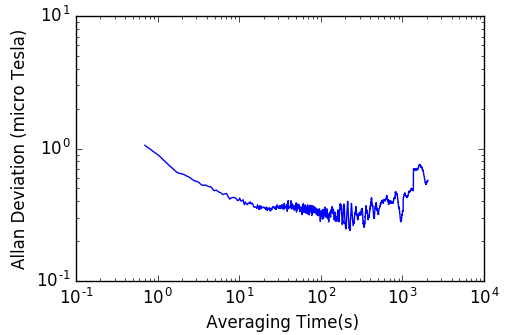
\includegraphics[width=0.6\linewidth]{figures/allan_plot}
\caption{Allan deviation vs. averaging time(s)}
\end{figure}
The Allan deviation can be express as
\begin{equation}
\sigma_y(\tau)=\sqrt{\sigma_y^2(\tau)}=Var_y(\tau)
\end{equation}
Where $\sigma_y$ is the Allan deviation, $\tau$ the time of each frequency estimate and $Var_y$ is the variance of the observed data points.
\begin{equation}
{\sigma_y^2(\tau)}=\frac{1}{2}(\bar{y}_{n+1}-\bar{y}_{n})
\end{equation}
where $\bar{y}_{n}$ is the fractional frequency average over the observation time $\tau$.
Allan deviation formula for sinusoidal waveform:
Suppose
\begin{equation}
y(t) = A\cos (\omega t + \phi)
\end{equation}
The average of this function over a time-interval  is
\begin{equation}
\bar{y}_{n}=\frac{2A}
{\tau \omega}
cos(\omega(t_n +\frac{\tau}{2})+\phi)sin(\frac{\omega \tau}{2})
\end{equation}
and
\begin{equation}
\bar{y}_{n+1}=\frac{2A}
{\tau \omega}
cos(\omega(t_{n+1} +\frac{\tau}{2})+\phi)sin(\frac{\omega \tau}{2})
\end{equation}
Now from equation(5.5) and (5.6) we can write
\begin{equation}
\bar{y}_{n+1}-\bar{y}_{n}=\frac{2A}
{\tau \omega}sin(\frac{\omega \tau}{2})[cos( \omega(t_{n+1} +\frac{\tau}{2})+\phi)-cos(\omega(t_n +\frac{\tau}{2})+\phi)]
\end{equation}
Thus Allan deviation can be written as

\begin{equation}
{\sigma_y^2(\tau)}=\frac{1}{2}(\bar{y}_{n+1}-\bar{y}_{n})=(\frac{4A}
{\tau \omega}sin^2(\frac{\omega \tau}{2}))^2 \sin^2     (\frac{\omega(t_{n+1} +t_{n}+\tau)}{2})+\phi)
\end{equation}
For a large number of randomly
distributed tk the average of the sine-squared function is
\begin{equation}
\sin^2    (\frac{\omega(t_{n+1} +t_{n}+\tau)}{2})+\phi)=\frac{1}{2}
\end{equation}
We therefore find that
\begin{equation}
{\sigma_y^2(\tau)}=(\frac{2A}
{\tau \omega}sin^2(\frac{\omega \tau}{2}))^2
\end{equation}

In FID mode, the resonance signal looks like a decaying sine wave. By fitting the NMOR signal with a damped sine wave the oscillation frequency has been extracted and finally this oscillation frequency has been translated to field.The Allan deviation of the measure field has been plotted in Figure 5.23.

  \section{study the effect of room temperature in magnetic field} 
  \begin{figure}[h]
\centering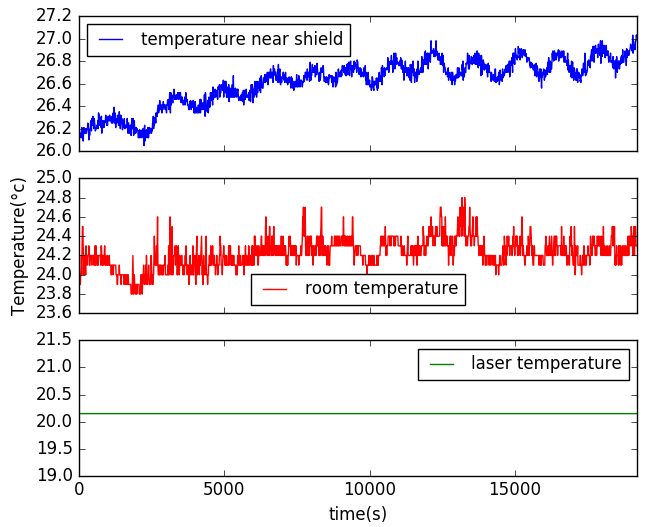
\includegraphics[width=0.8\linewidth]{figures/temp_.png}
\caption{Temperature measurement\label{temperature}}
\end{figure}
  \begin{figure}[h]
\centering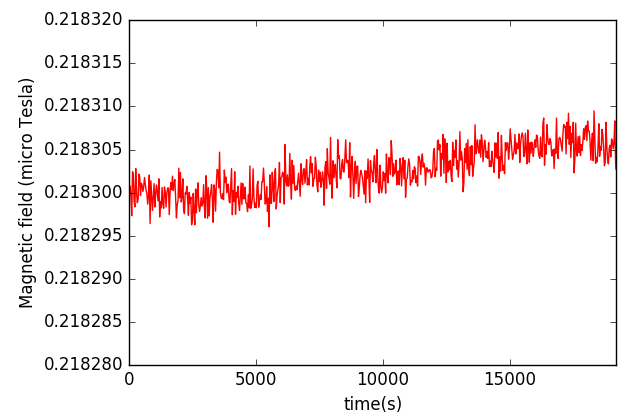
\includegraphics[width=0.8\linewidth]{figures/field_.png}
\caption{Field measurement\label{field}}
\end{figure}
 \begin{figure}[h]
\centering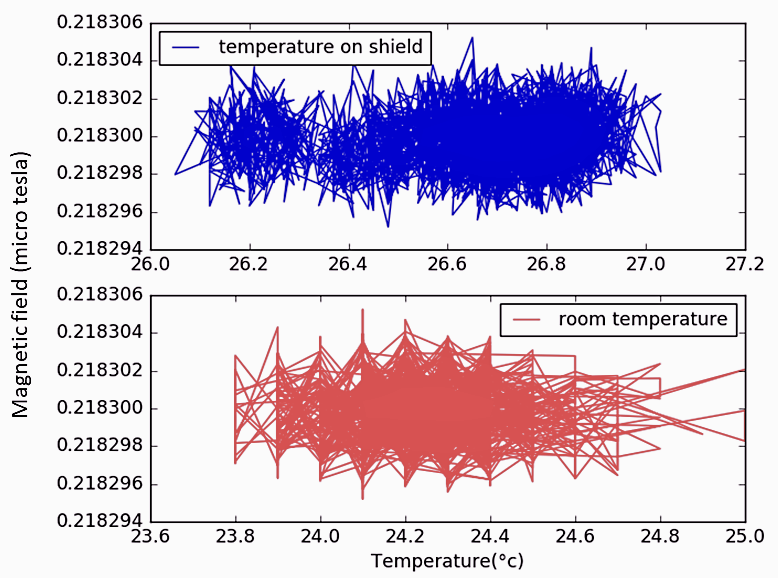
\includegraphics[width=0.8\linewidth]{figures/field_vs_temp.png}
\caption{Field vs. temperature\label{field_vs_temp}}
\end{figure}
\newpage
\section{Study magnetometer performance with tilted field} 
\label{sec:tilted-results}
 \begin{figure}
    \centering
    \begin{subfigure}[b]{0.45\textwidth}
        \centering
        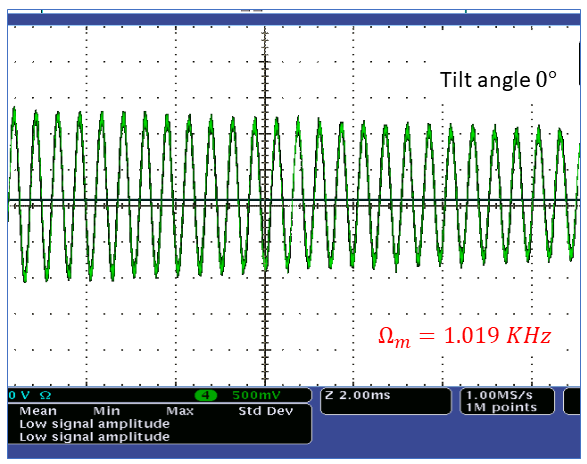
\includegraphics[width=\textwidth]{figures/tilt1.png}
        \caption{}
        \label{fig:tilt_0_degree}
    \end{subfigure}
    \hfill
    \begin{subfigure}[b]{0.45\textwidth}
        \centering
        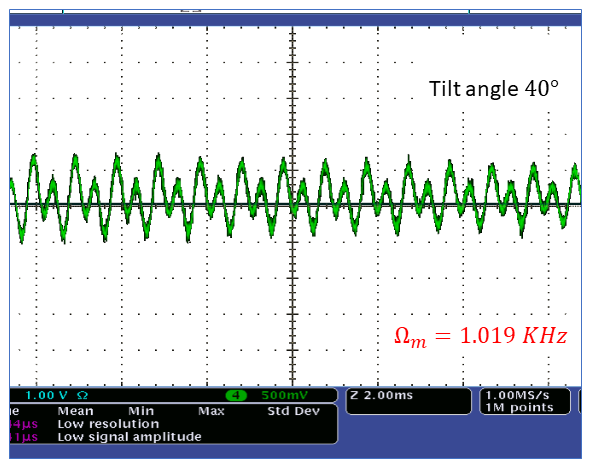
\includegraphics[width=\textwidth]{figures/tilt2.png}
        \caption{}
        \label{fig:tilt_40_degree}
    \end{subfigure}
    \begin{subfigure}[b]{0.45\textwidth}
        \centering
        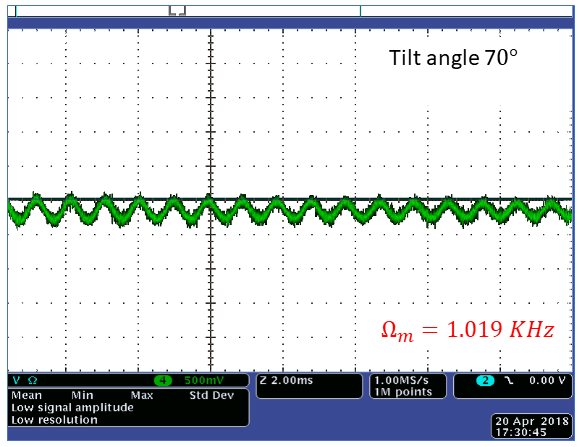
\includegraphics[width=\textwidth]{figures/tilt3.png}
        \caption{}
        \label{fig:tilt_70_degree}
    \end{subfigure}
     \hfill
    \begin{subfigure}[b]{0.45\textwidth}
        \centering
        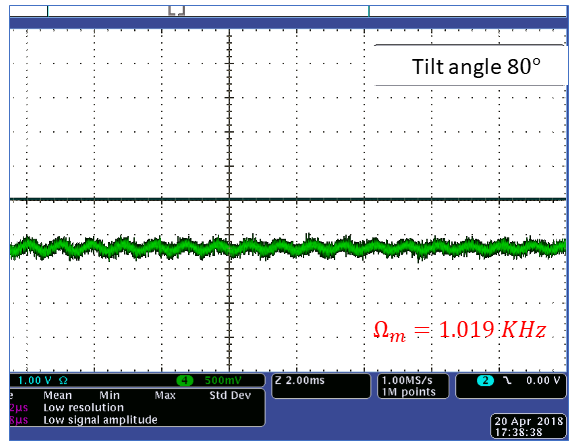
\includegraphics[width=\textwidth]{figures/tilt4.png}
        \caption{}
        \label{fig:tilt_80_degree}
    \end{subfigure}
    \caption{Optical rotation as a function of time at $\Omega_L$ in the yz plane for different tilt angle.\label{fig:optical-rotation-different-angle}}
\end{figure}
